\appendix
\chapter{Supplementary Tables}
\label{app:supplementary-tables}

\section{Batch Pricing Table}
\label{app:batch-pricing-table}

\begin{table}[htbp]
    \centering
    \caption{Batch-API prices per one million tokens (USD) for all models in \texttt{config/models.yaml} as of 16~March~2026.}
    \label{tab:batch-pricing-examples}
    \begin{tabular}{lll}
        \toprule
        Model & Input price & Output price \\
        \midrule
        \texttt{gpt-5.4-2026-03-05}      & 1.25  & 7.50  \\
        \texttt{gpt-5.4}                 & 1.25  & 7.50  \\
        \texttt{gpt-5.2}                 & 0.875 & 7.00  \\
        \texttt{gpt-5.2-pro}             & 10.50 & 84.00 \\
        \texttt{gpt-5.1}                 & 0.625 & 5.00  \\
        \texttt{gpt-5}                   & 0.625 & 5.00  \\
        \texttt{gpt-5-pro}               & 7.50  & 60.00 \\
        \texttt{gpt-5-mini}              & 0.125 & 1.00  \\
        \texttt{gpt-5-nano}              & 0.025 & 0.20  \\
        \texttt{gpt-4.1}                 & 1.00  & 4.00  \\
        \texttt{gpt-4.1-mini}            & 0.20  & 0.80  \\
        \texttt{gpt-4.1-nano}            & 0.05  & 0.20  \\
        \texttt{gpt-4o-2024-05-13}       & 2.50  & 7.50  \\
        \texttt{gpt-4o}                  & 1.25  & 5.00  \\
        \texttt{gpt-4o-mini}             & 0.075 & 0.30  \\
        \texttt{o1}                      & 7.50  & 30.00 \\
        \texttt{o1-pro}                  & 75.00 & 300.00 \\
        \texttt{o1-mini}                 & 0.55  & 2.20  \\
        \texttt{o3}                      & 1.00  & 4.00  \\
        \texttt{o3-pro}                  & 10.00 & 40.00 \\
        \texttt{o3-mini}                 & 0.55  & 2.20  \\
        \texttt{o3-deep-research}        & 5.00  & 20.00 \\
        \texttt{o4-mini}                 & 0.55  & 2.20  \\
        \texttt{o4-mini-deep-research}   & 1.00  & 4.00  \\
        \texttt{gemini-3-flash-preview}           & 0.25  & 1.50  \\
        \texttt{gemini-2.5-flash}                 & 0.15  & 1.25  \\
        \texttt{gemini-2.5-flash-preview-09-2025} & 0.15  & 1.25  \\
        \texttt{gemini-2.0-flash}                 & 0.05  & 0.20  \\
        \texttt{gemini-2.5-pro}                   & 0.625 & 5.00  \\
        \texttt{claude-opus-4-6}   & 2.97 & 14.88 \\
        \texttt{claude-opus-4-5}   & 2.97 & 14.88 \\
        \texttt{claude-opus-4-1}   & 8.92 & 44.63 \\
        \texttt{claude-opus-4}     & 8.92 & 44.63 \\
        \texttt{claude-sonnet-4-6} & 1.78 & 8.92  \\
        \texttt{claude-sonnet-4-5} & 1.78 & 8.92  \\
        \texttt{claude-sonnet-4}   & 1.78 & 8.92  \\
        \texttt{claude-haiku-4-5}  & 0.59 & 2.97  \\
        \texttt{claude-3.5-haiku}  & 0.40 & 2.00  \\
        \bottomrule
    \end{tabular}
\end{table}

\section{Per-metric ranking charts (monitoring snapshot)}
\label{app:per-metric-ranking-charts}

The following charts are supplementary visualizations of the exported monitoring snapshot from \texttt{assets/metrics\_export/}. They complement, but do not replace, the main decision tables in Chapters~\ref{ch:cost-deployment-utility} and~\ref{chap:system-architecture}.
Formal metric definitions and formulas are given in Chapter~\ref{ch:drift} (Section~\ref{sec:classification-metrics}); interpretation of metric movement for operational decisions is provided in Chapter~\ref{chap:system-architecture} and the episode narrative in Chapter~\ref{chap:degradation-case-study}.

\IfFileExists{assets/fig-metric-accuracy.png}{%
\begin{figure}[htbp]
    \centering
    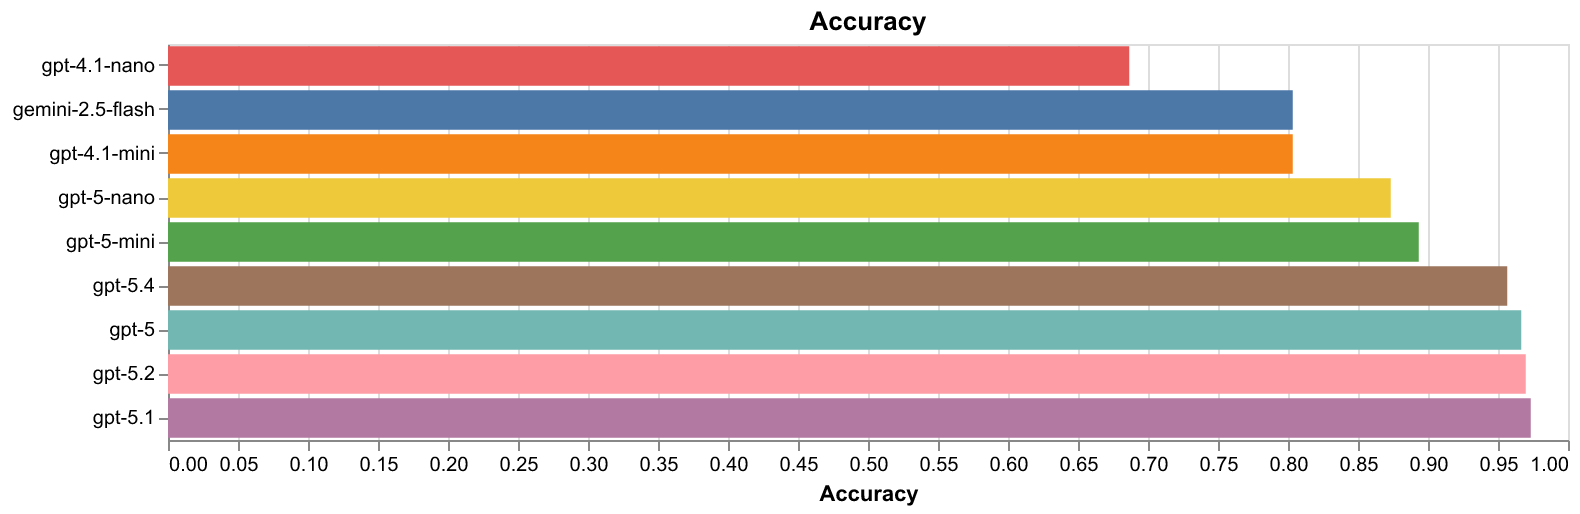
\includegraphics[width=\linewidth]{assets/fig-metric-accuracy.png}
    \caption{Per-model ranking by accuracy on $\mathcal{D}_n$.}
\end{figure}
}{}

\IfFileExists{assets/fig-metric-balanced_accuracy.png}{%
\begin{figure}[htbp]
    \centering
    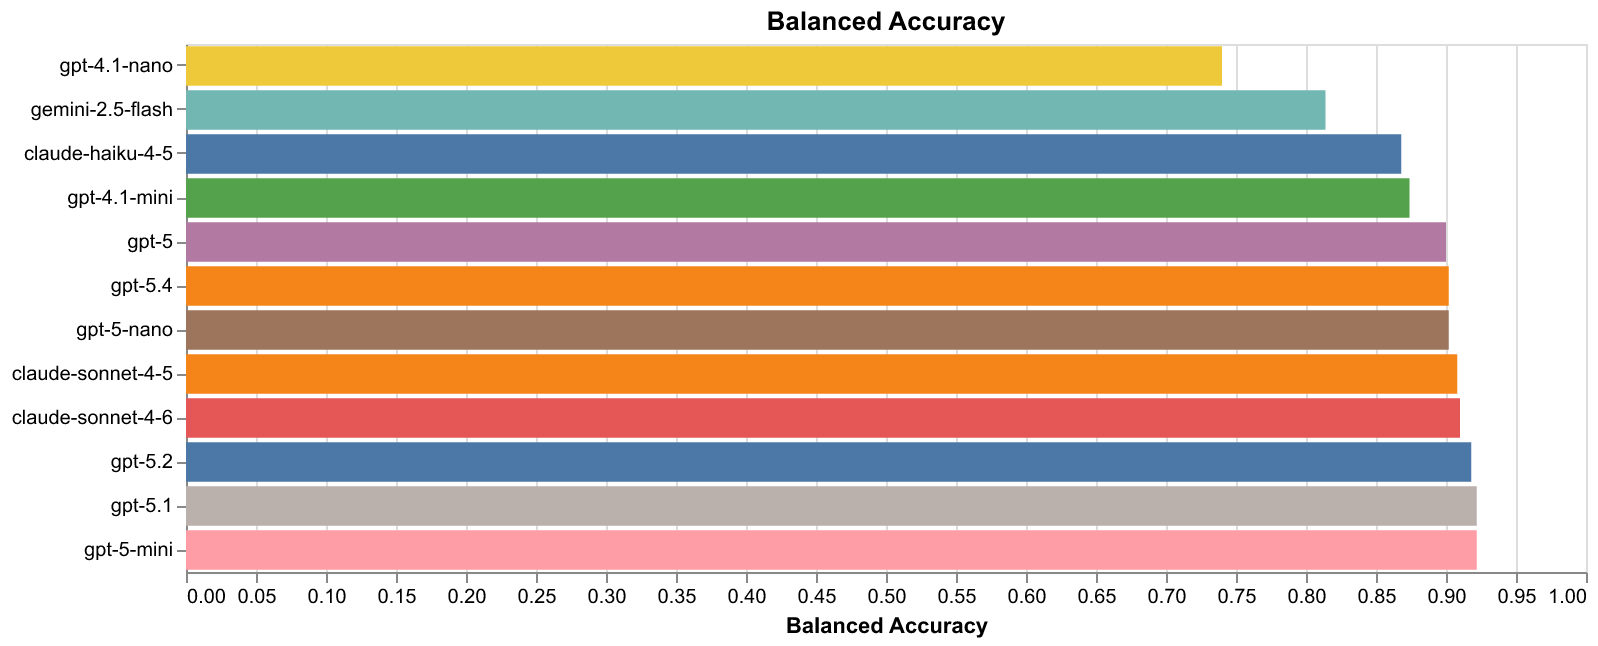
\includegraphics[width=\linewidth]{assets/fig-metric-balanced_accuracy.png}
    \caption{Per-model ranking by balanced accuracy on $\mathcal{D}_n$.}
\end{figure}
}{}

\IfFileExists{assets/fig-metric-f1.png}{%
\begin{figure}[htbp]
    \centering
    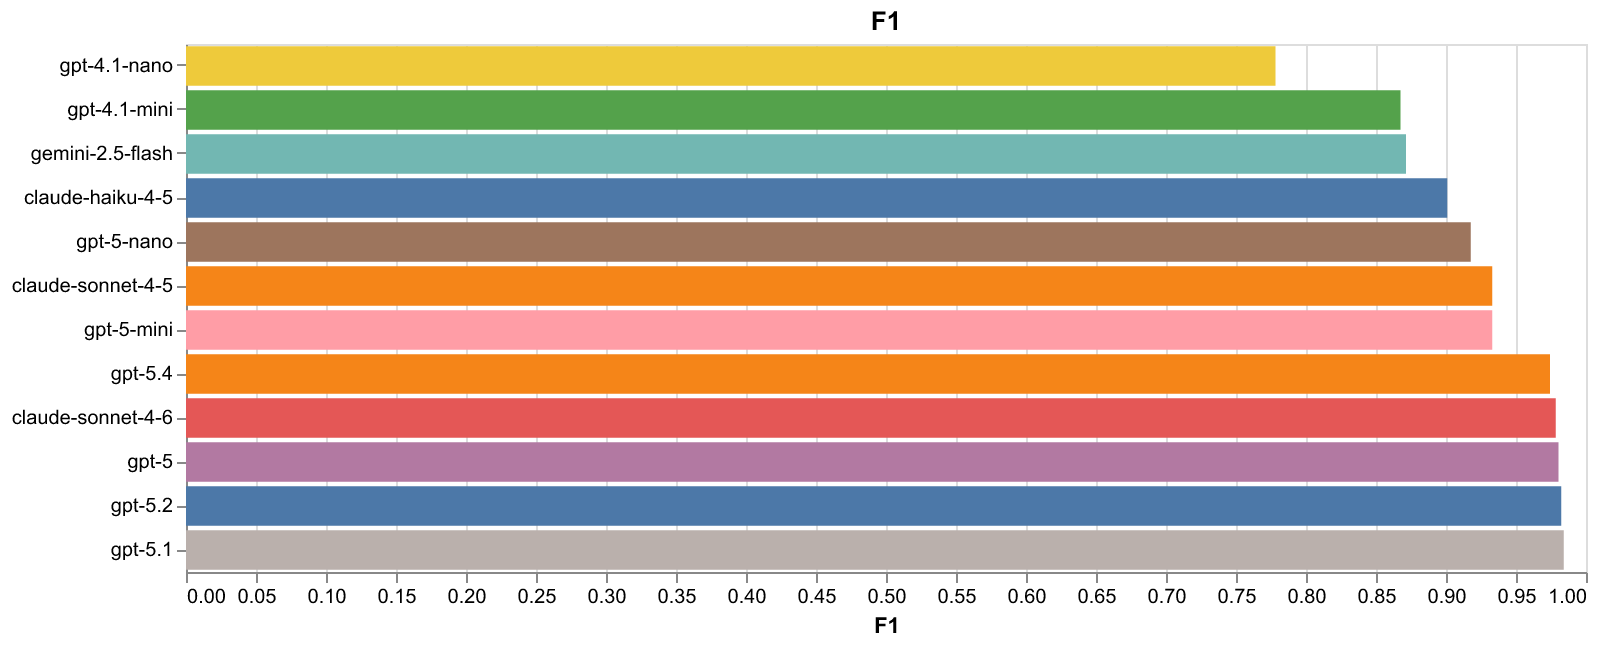
\includegraphics[width=\linewidth]{assets/fig-metric-f1.png}
    \caption{Per-model ranking by F1 score on $\mathcal{D}_n$.}
\end{figure}
}{}

\IfFileExists{assets/fig-metric-pr_auc.png}{%
\begin{figure}[htbp]
    \centering
    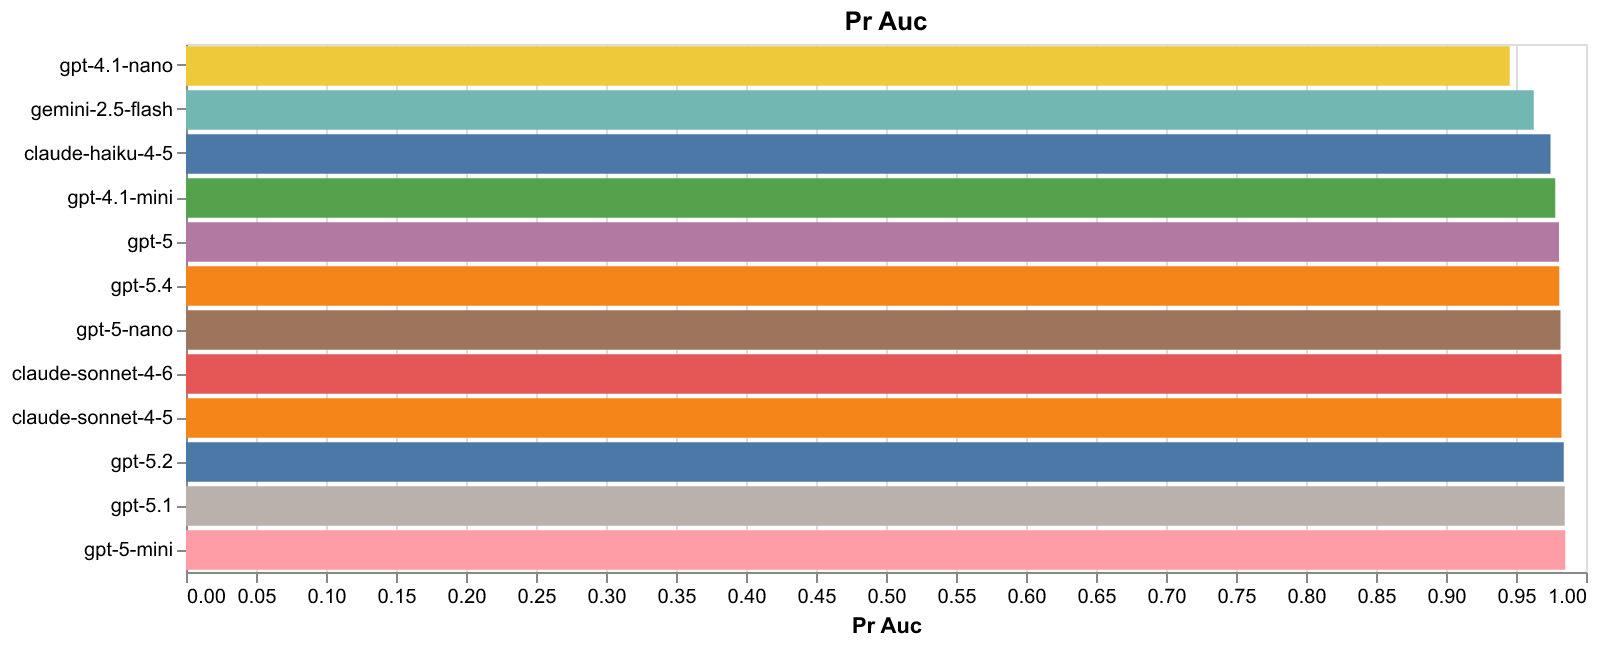
\includegraphics[width=\linewidth]{assets/fig-metric-pr_auc.png}
    \caption{Per-model ranking by PR--AUC on $\mathcal{D}_n$.}
\end{figure}
}{}

\IfFileExists{assets/fig-metric-precision.png}{%
\begin{figure}[htbp]
    \centering
    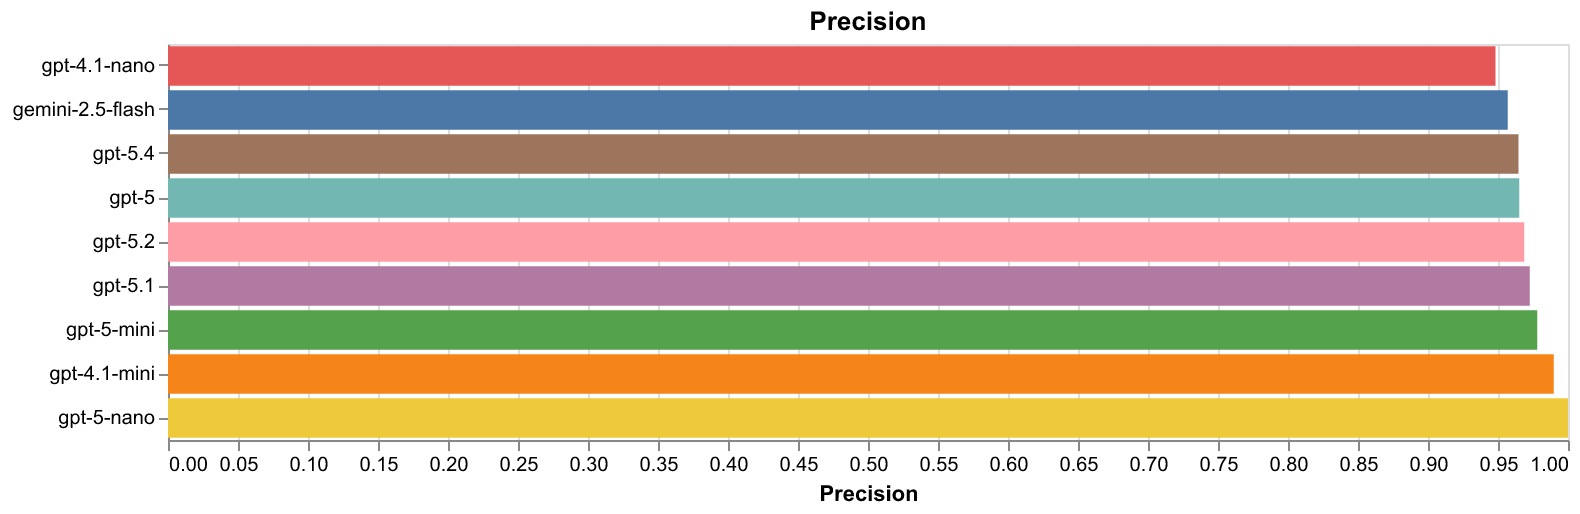
\includegraphics[width=\linewidth]{assets/fig-metric-precision.png}
    \caption{Per-model ranking by precision on $\mathcal{D}_n$.}
\end{figure}
}{}

\IfFileExists{assets/fig-metric-recall.png}{%
\begin{figure}[htbp]
    \centering
    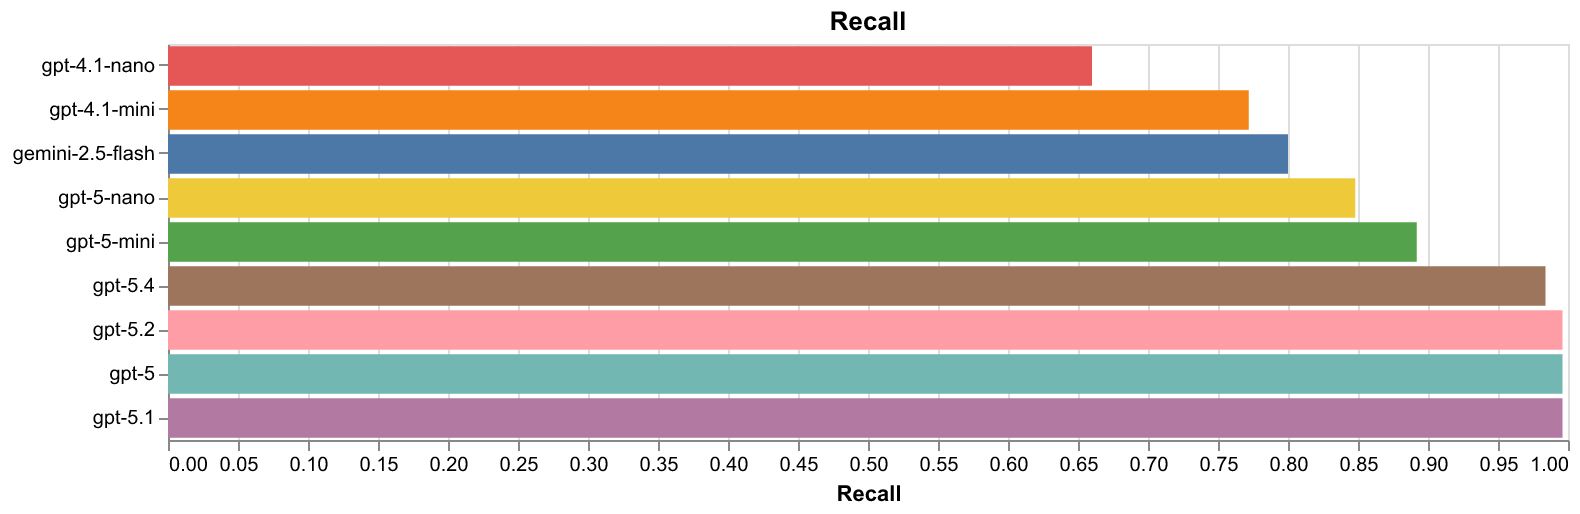
\includegraphics[width=\linewidth]{assets/fig-metric-recall.png}
    \caption{Per-model ranking by recall on $\mathcal{D}_n$.}
\end{figure}
}{}

\IfFileExists{assets/fig-metric-specificity.png}{%
\begin{figure}[htbp]
    \centering
    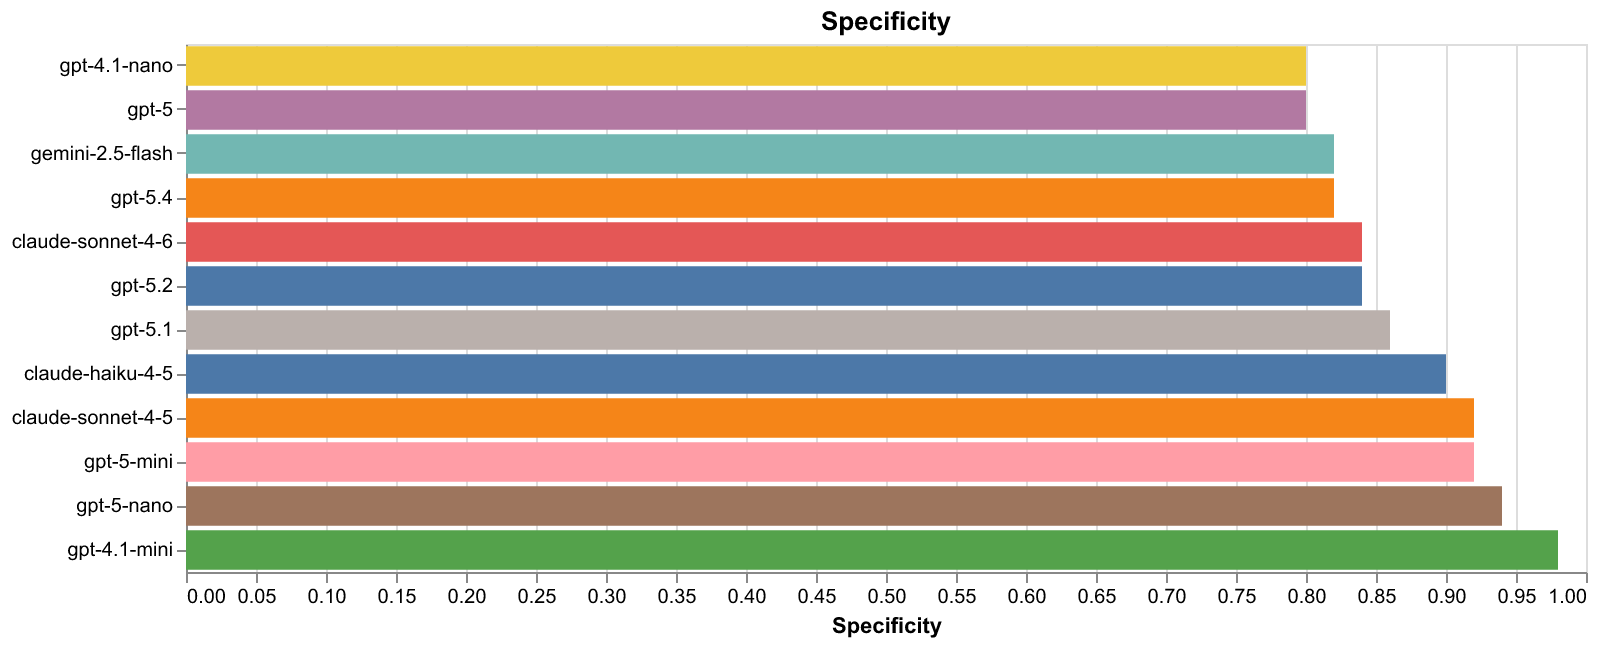
\includegraphics[width=\linewidth]{assets/fig-metric-specificity.png}
    \caption{Per-model ranking by specificity on $\mathcal{D}_n$.}
\end{figure}
}{}



{}

